\chapter{Introducción específica} % Main chapter title

\label{Chapter2}

%----------------------------------------------------------------------------------------
%	SECTION 1
%----------------------------------------------------------------------------------------
%En este capítulo se presentan las tecnologías utilizadas e incorporadas en este trabajo. 

En este capítulo se explica el funcionamiento general del sistema implementado y se brinda una introducción a las diferentes tecnologías utilizadas en este trabajo.

\section{Funcionamiento general del sistema}

Este trabajo presenta una propuesta de solución a partir del desarrollo de un prototipo mínimo viable de un sistema IoT para integrar, centralizar y unificar resultados de una red de sensores y actuadores, mediante un sistema web de monitoreo y control, así como la construcción de módulos propios para dicha tarea, sin la necesidad de una conexión a Internet para su funcionamiento. 

Todos estos componentes trabajan en conjunto para brindar al cliente una solución tecnológica que sirva como herramienta visualmente amigable y que pueda ser el soporte en las tareas de gestión de consumo eléctrico. Para lograrlo, se desarrollaron módulos que integran \emph{software} y \emph{hardware}, estos hacen posible la adquisición de datos de sensores y actuadores ubicados en distintos puntos de una vivienda, conectados a una red local vía Wi-Fi. Cada lectura de los sensores permite el envío de datos a un servidor central local mediante el protocolo MQTT por vía inalámbrica, siendo el módulo principal local el responsable de registrar los valores de los sensores ante cualquier corte de Internet. La figura \ref{fig:diagrama1} ilustra el diagrama de componentes del sistema y la lógica de conexión.

\begin{figure}[htbp]
	\centering
	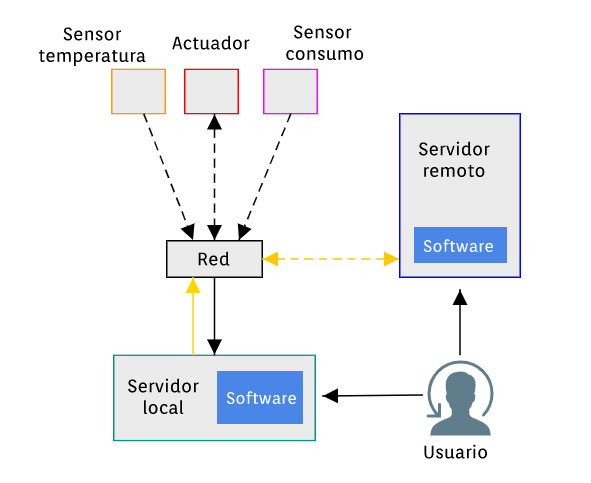
\includegraphics[width=0.9\textwidth]{./Figures/bloques.png}
	\caption{Diagrama de bloques del sistema.}

	\label{fig:diagrama1}
\end{figure}

El sistema tiene la capacidad de permitir el acceso por medio de cualquier dispositivo que cuente con un navegador web y con conectividad a Internet a cualquier usuario, ya sea desde dentro de la red local o desde fuera. Para alcanzar esta funcionalidad, fue necesario desarrollar un módulo de \emph{software} que permita la replicación de datos desde la red local hacia un broker remoto ubicado en la nube. La necesidad de replicación de los datos hacia la nube solo se da mientras exista conexión a Internet. Para los casos de corte de Internet, el módulo replicador enviará los datos de forma automática la próxima vez que detecte el servicio.% de conexión a Internet. 

Los componentes claves dentro de la solución propuesta y que se integran en la arquitectura IoT usada en el proceso de desarrollo son: 


\begin{itemize}
\item Dispositivos IoT: son los módulos diseñados a partir de la integración de \emph{software}, \emph{firmware} y \emph{hardware}; es posible conectarlos de forma inalámbrica a una red más amplia.
\item Redes: los routers domésticos, puntos de acceso y las configuraciones de las redes o las puertas de enlaces son los responsables de conectar varios dispositivos IoT a la nube.
\item Nube: servidores remotos en centros de datos que consolidan y almacenan la información con seguridad. Son servicios utilizados en el trabajo para garantizar el acceso remoto de usuarios al sistema.
\end{itemize}

\section{Servicios en la nube}

El \emph{Cloud Computing} o servicios en la nube cobra cada vez más relevancia en las empresas debido, principalmente, a la ventaja de no tener que hacer grandes inversiones en infraestructuras que mantengan aplicaciones, plataformas o servidores propios.

Los servicios en la nube se clasifican en:

\begin{itemize}
\item Infraestructura como servicio (IaaS): esta categoría ofrece servicios de infraestructura, entre ellos está la distribución de recursos de computación y almacenamiento cuyos precios varían de acuerdo al consumo realizado. Las empresas que los contratan nunca ven el equipo físico, pero sí pueden tener acceso a ellos al momento de usar el servicio deseado \citep{BOOK:2}.

%Ejemplo de IaaS:

%\begin{itemize}
%\item Amazon Web Services
%\item Microsoft Azure
%\item Google Cloud Platform
%\end{itemize}

%\vspace{0.5cm}

\item Plataforma como servicio (PaaS): este servicio ofrece plataformas de desarrollo sin necesidad de adquirir tecnología de costo muy elevado. El \emph{hardware} y el \emph{software} en este modelo es administrado por el proveedor del servicio, además de que los desarrolladores no se preocupan por el rendimiento del hardware ni por las actualizaciones del sistema, ya que todo lo realiza el proveedor \citep{BOOK:2}.
 
%Ejemplos de PaaS:

%\begin{itemize}
%\item AWS Elastic Beanstalk
%\item Azure App Service
%item Google App Engine

%\end{itemize}

%\vspace{0.5cm}


\item \emph{Software} como servicio (SaaS): constituye el modelo más utilizado porque, además de brindar servicio de \emph{software}, ofrece también el almacenamiento de la información. Este modelo permite simplicidad de integración y escalabilidad \citep{BOOK:2}. 

%Ejemplos de SaaS:

%\begin{itemize}
%\item Microsoft Office 365
%\item Aplicaciones web de Google
%\end{itemize}

%\vspace{0.5cm}

\end{itemize}

En la figura \ref{fig:servicios} se muestra una representación gráfica para diferenciar las capas y su orientación para cada modelo de servicio.



%\vspace{1.5cm}

\begin{figure}[htbp]
	\centering
	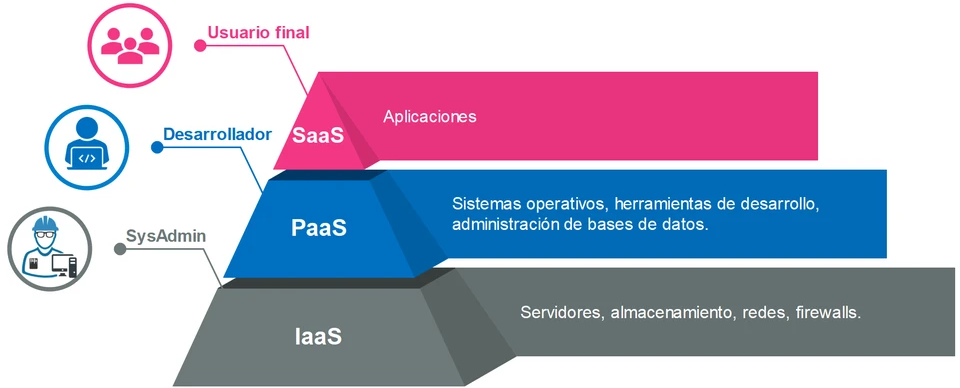
\includegraphics[width=.9\textwidth]{./Figures/servicios.png}
	\caption{Tipos de servicio y orientación por rol \protect\footnotemark.}

	\label{fig:servicios}
\end{figure}

\footnotetext{Imagen tomada de \url{https://openwebinars.net/blog/tipos-de-cloud-computing/}}

%\vspace{1cm}

Para el trabajo se usó el servicio tipo PaaS en la creación y configuración del broker remoto así como para el almacenamiento de la aplicación web y para la gestión de la base de datos.


%Para el trabajo se consideró el servicio de \emph{cloud computing} tipo PaaS, porque permite la creación y configuración del broker remoto, el servidor Apache para la aplicación web y el gestor de base de datos MySQL.

El plan utilizado se divide en dos categorías, la primera está definida por el servicio del servidor web para alojar la aplicación web de monitoreo y control (réplica) y la segunda por el servicio del broker remoto que permite la comunicación directa con el broker local. La comunicación entre ambos servicios se hace mediante el protocolo MQTT utilizando la biblioteca  \emph{Eclipse Paho JavaScript Client}, se puede encontrar mayor información en su página oficial \citep{WEBSITE:41}. 

Las principales características  del servicio contratado para la implementación del sistema de monitoreo se muestran en la tabla \ref{tab:serverweb} y las características del servicio para el broker remoto se muestran en la tabla  \ref{tab:brokerremoto}.


\begin{table}[h]
	\centering
	\caption[Características del servicio en la nube]{Características del servicio en la nube.}
	\begin{tabular}{p{7cm} p{5cm} }    
		\toprule
		\textbf{Característica} 	 & \textbf{Detalle}  \\
		\midrule
		Sistema operativo  & GNU/Linux Centos\\		
		Espacio de almacenamiento & 1000 MB \\
		Transferencia mensual  & 10 GB\\				
		Cantidad base de datos 	  & ilimitados\\
		Acceso FTP 	  & sí\\
		Backup diario y semanal 	  & sí\\
		Soporte 24/7 	  & sí\\
		Seguridad - Firewall	  & sí\\
		Certificados SSL/TLS	  & sí\\
		PHP	  & V7 y V8\\
		MySQL	  & sí\\
		phpMyAdmin	  & sí\\
		Cron Jobs	  & sí\\
		\bottomrule
		\hline
	\end{tabular}
	\label{tab:serverweb}
\end{table}

%%%%%%%%%%%%%%%%%%%%%%%%%%%%%%%%%%%%%%%%%%%%%%%%%%%%%

\begin{table}[h]
	\centering
	\caption[Características del broker remoto]{Características del broker remoto.}
	\begin{tabular}{p{5cm} p{7cm} }    
		\toprule
		\textbf{Característica} 	 & \textbf{Detalle}  \\
		\midrule
		Conexiones activas  & 200\\		
		Mensajes por segundo & 10 k \\
		Interface  & MQTT interface, HTTP interface\\		
		Compatibilidad & arduino, javaScript, processing, ruby \\		
		Deployment 	  & por instancias\\
		Envíos y recepción de datos & objetos codificados JSON\\
		
		\bottomrule
		\hline
	\end{tabular}
	\label{tab:brokerremoto}
\end{table}




%En la figura \ref{fig:capas-servicios} se muestran las capas de cada servicio descrito y el acceso que el cliente tiene con cada modelo (capas de color verde).

%\begin{figure}[htbp]
%	\centering
%	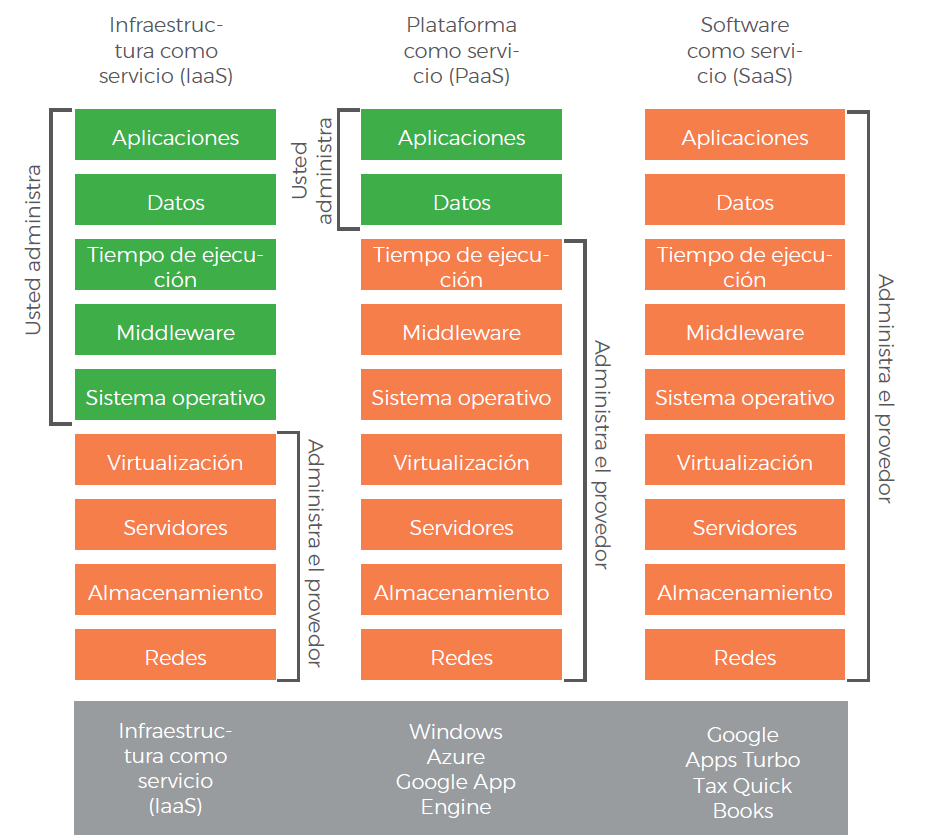
\includegraphics[width=.8\textwidth]{./Figures/capas-servicios.png}
%	\caption{Infraestructura por capas según el servicio  \citep{BOOK:2}.}

%	\label{fig:capas-servicios}
%\end{figure}

%\footnotetext{Imagen tomada del libro \textit{Cloud Computing for Pymes}. \citep{BOOK:1}}}



\section{Protocolo MQTT}

MQTT  (\textit{Message Queue Telemetry Transport}) es un protocolo de red ligero de mensajería estándar para IoT. Está diseñado como un transporte de mensajería extremadamente liviano y se utiliza en una amplia variedad de industrias, como la automotriz, las telecomunicaciones, el petróleo y el gas, entre otros  \citep{WEBSITE:4}. 

Para construir una red usando MQTT es necesario entender los conceptos que se utilizan para crear una red IoT: 

\begin{itemize}
\item El broker MQTT: el servidor o broker es el programa que se encarga de recepcionar los mensajes enviados por los clientes y distribuirlos entre sí en un sistema publicador-suscriptor. Los clientes envían periódicamente paquetes y esperan la respuesta del broker, como se ilustra con la figura \ref{fig:broker}. 

\begin{figure}[htbp]
	\centering
	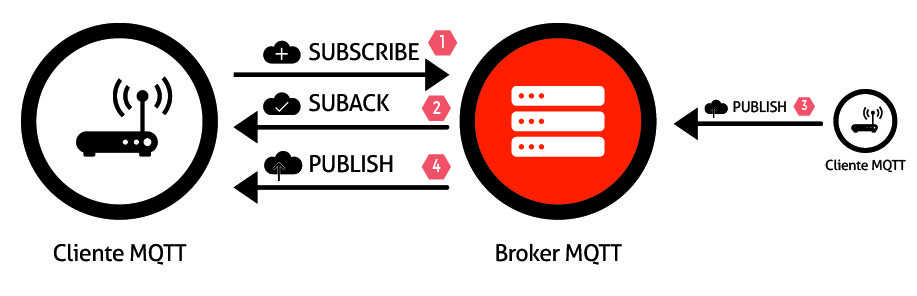
\includegraphics[width=.75\textwidth]{./Figures/broker.jpg}
	\caption{Funcionamiento del broker MQTT \protect\footnotemark.}

	\label{fig:broker}
\end{figure}

\footnotetext{Imagen tomada de \url{https://www.factor.mx/portal/base-de-conocimiento/mqtt/}}

El broker MQTT usado en el trabajo es Eclipse Mosquitto, por ser de código abierto.

%\vspace{1cm}
%\vspace{1cm}
\item Comunicación MQTT: es la función de transporte de mensajes entre dispositivos IoT. El protocolo generalmente se ejecuta sobre TCP / IP ; sin embargo, cualquier protocolo de red que proporcione conexiones bidireccionales ordenadas y sin pérdidas puede admitir MQTT. Está diseñado para conexiones con ubicaciones remotas donde existen restricciones de recursos o el ancho de banda de la red es limitado \citep{WEBSITE:3}. Su modelo de comunicación se puede ver en la figura \ref{fig:mqtt}.

%\vspace{0.5cm}



La comunicación MQTT puede estar cifrada mediante TLS (\emph{Transport Layer Security}) y contar con credenciales de acceso para el control de los canales de envío y recepción. Al broker se le puede conectar un sinfín de dispositivos como teléfonos móviles, computadoras, sensores, actuadores, lámparas, relojes, bombas de agua, refrigeradores, cocinas y mucho más. 

\begin{figure}[htbp]
	\centering
	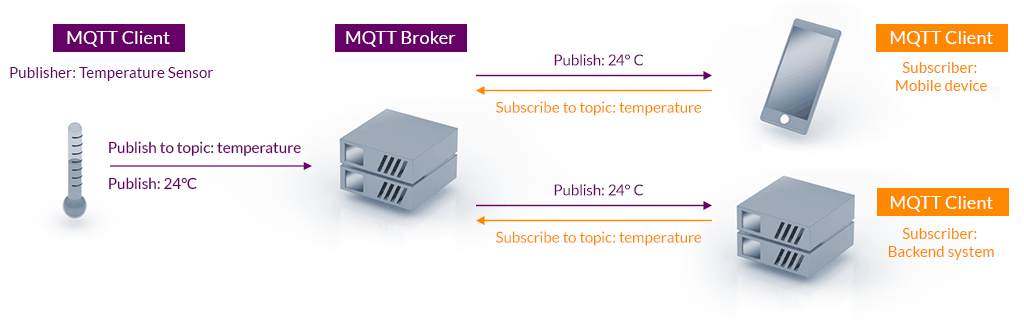
\includegraphics[width=0.95\textwidth]{./Figures/mqtt.png}
	\caption{Ejemplo de funcionamiento del protocolo MQTT \protect\footnotemark.}
	\label{fig:mqtt}
\end{figure}

\footnotetext{Imagen tomada de \url{https://mqtt.org/}}

\end{itemize}

%\section{Elementos del broker MQTT}


%\begin{itemize}
%\item Cliente: un dispositivo que puede publicar mensajes, suscribirse para recibir mensajes, o ambos.
%\item Broker: es el servidor que acepta mensajes publicados por clientes y los difunde entre los clientes suscritos.
%\item Publicar: cuando un cliente envía un mensaje al broker usando un tópico.
%\item Tópico: los mensajes deben estar etiquetados con algún tópico o tema. Los clientes se suscriben a tópicos específicos, de manera que solo reciben los mensajes publicados con dichos tópicos. 
%\end{itemize}


\section{Eclipse Mosquitto} 
Es un agente de mensajes de código abierto (con licencia EPL / EDL) cuya versión 2.0.14 implementa las versiones 5.0, 3.1.1 y 3.1 del protocolo MQTT. Mosquitto es liviano y adecuado para su uso en todos los dispositivos, desde computadoras de placa única de baja potencia hasta servidores completos \citep{WEBSITE:5}.

%El protocolo MQTT proporciona un método ligero para realizar mensajes mediante un modelo de publicación / suscripción. Esto lo hace adecuado para la mensajería de Internet de las cosas, como con sensores de baja potencia o dispositivos móviles como teléfonos, computadoras integradas o microcontroladores \citep{WEBSITE:5}.

Mosquitto es parte de la Fundación Eclipse \citep{WEBSITE:5}, es un proyecto de IoT \citep{WEBSITE:39} y está patrocinado por la compañía Cedalo \citep{WEBSITE:40}. 

\section{Componentes del módulo principal} 

El hardware del módulo principal integra la placa raspberry Pi 4 modelo B de 8 GB como placa base. La Raspberry Pi es una serie de ordenador de placa reducida, ordenador de placa única u ordenador de placa simple (SBC) de bajo costo desarrollado en el Reino Unido por la Raspberry Pi Foundation \citep{WEBSITE:6}.

La placa Raspberry Pi 4 es una pequeña computadora de escritorio de doble pantalla con opciones de salida en 4K, se puede usar como cerebro de robot, centro de hogar inteligente, centro multimedia, núcleo de IA (inteligencia artificial) en red y mucho más. La figura \ref{fig:rpi4} muestra sus principales especificaciones.

Las especificaciones técnicas de la computadora Raspberry Pi 4 son \citep{WEBSITE:7}:

\begin{itemize}
\item Broadcom BCM2711, SoC de 64 bits Cortex-A72 de cuatro núcleos (ARM V8) a 1,5 GHz.
\item SDRAM LPDDR4-3200 de 2 GB, 4 GB u 8 GB (según el modelo).
\item 2,4 GHz y 5,0 GHz IEEE 802.11ac inalámbrica, Bluetooth 5.0.
\item Gigabit Ethernet, 2 puertos USB 3.0 y 2 puertos USB 2.0.
\item Cabecera GPIO estándar Raspberry Pi de 40 pines (totalmente compatible con las placas anteriores).
\item Puertos micro-HDMI (hasta 4kp 60 compatible).
\item Ranura para tarjeta microSD para cargar el sistema operativo y el almacenamiento de datos.
\item 5 VCC a través del conector USB-C (mínimo 3 A).
\item 5 VCC a través del encabezado GPIO (mínimo 3 A).
\item Power over Ethernet (PoE) habilitado (requiere PoE HAT separado).
\item Temperatura de funcionamiento ambiente: 0 °C - 50 °C.
\end{itemize}

%%%%%%%%%%%%%%%%%%%%%%%%%%%%%%%%%%%%%%%%%%%%%%%%%%%%%%%%%%%%%%%%%%%
\begin{figure}[htbp]
	\centering
	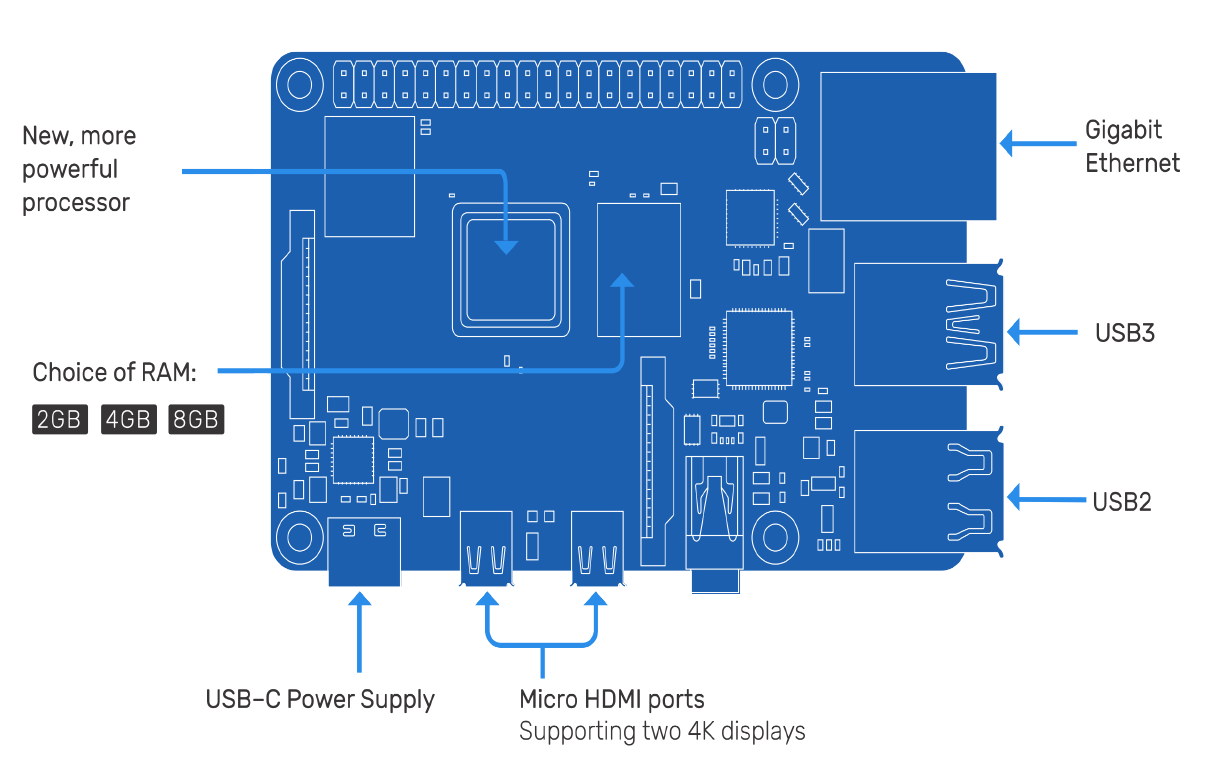
\includegraphics[width=1.0\textwidth]{./Figures/rpi4.png}
	\caption{Computadora Raspberry Pi 4 \protect\footnotemark. \citep{WEBSITE:7}}

	\label{fig:rpi4}
\end{figure}

\footnotetext{Imagen de \url{https://www.raspberrypi.com/products/raspberry-pi-4-model-b/specifications/}}

%\vspace{1cm}

%%%%%%%%%%%%%%%%%%%%%%%%%%%%%%%%%%%%%%%%%%%%%%%%
\subsection{Alimentación, gabinete y unidad de almacenamiento}

La fuente de alimentación para la Raspberry Pi 4 es de 3 A como se aprecia en la figura \ref{fig:placarpi4}. La unidad de almacenamiento contiene una unidad de memoria extraíble microSD de 64 GB y de clase 10 para garantizar alta velocidad de lectura y escritura durante el procesamiento.
% La figura \ref{fig:microsd} muestra la microSD del módulo.

\begin{figure}[htpb]
\centering 
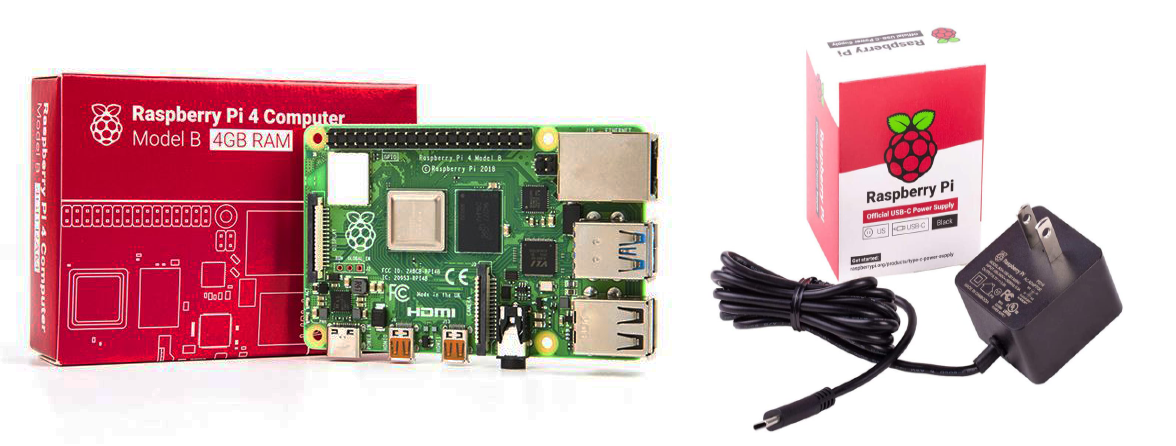
\includegraphics[width=0.8\textwidth]{./Figures/placa.png}
\caption{Mainboard y fuente de alimentación del servidor.}
\label{fig:placarpi4}
\end{figure}
%\begin{figure}[htpb]
%\centering 
%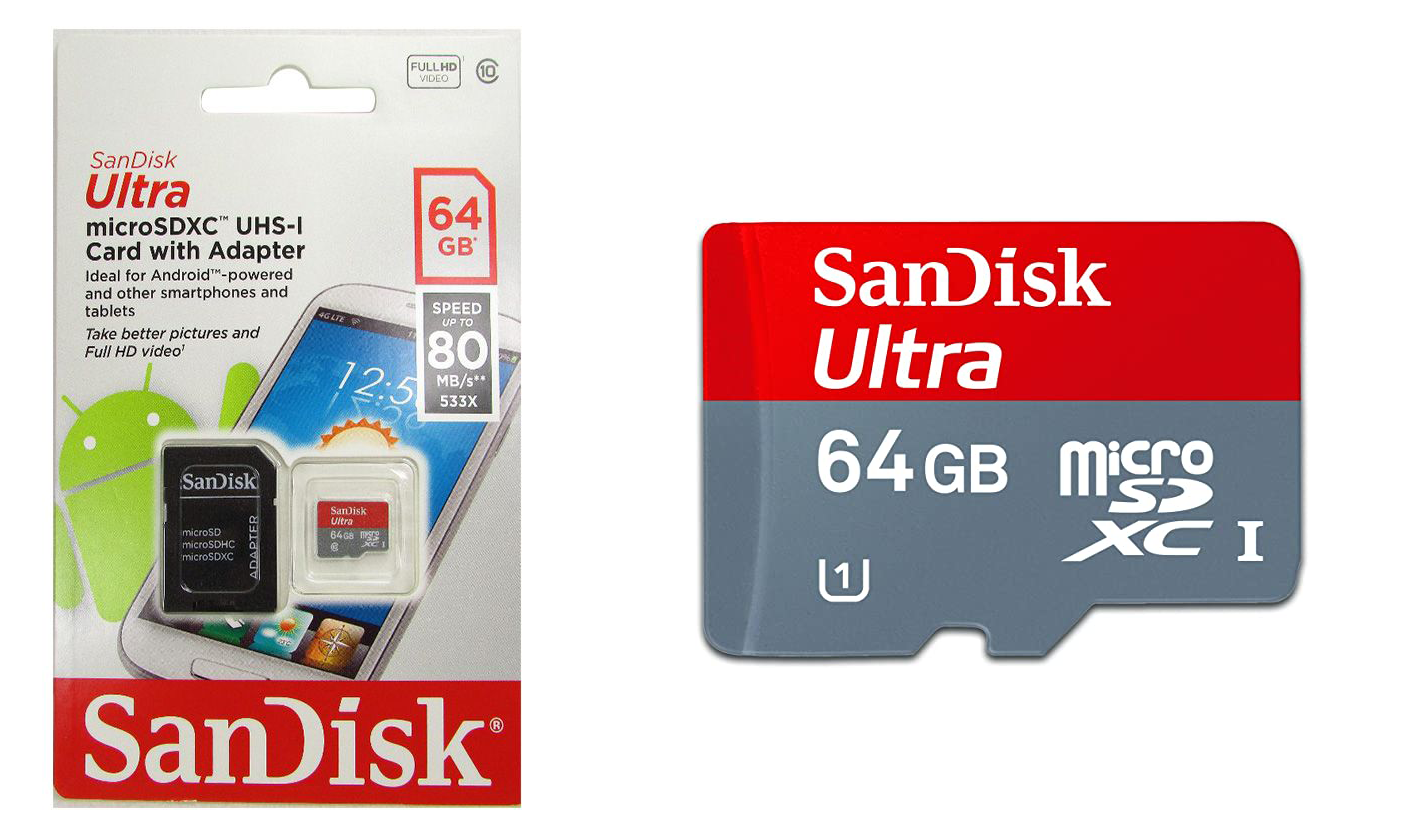
\includegraphics[width=0.7\textwidth]{./Figures/card.png}
%\caption{Tarjeta de almacenamiento del servidor local.}
%\label{fig:microsd}
%\end{figure}
El case Argon One Pi4 V2 es el gabinete usado para este trabajo como componente para la integración de elementos del módulo principal. La figura \ref{fig:armado} muestra las partes del gabinete.  
\vspace{1.5cm}

%Características del gabinete \citep{WEBSITE:16}:

%\begin{itemize}
%\item Tiene una placa Raspberry Pi Sata, que está diseñada para maximizar las transferencias de datos de alta velocidad para el uso de SSD Raspberry Pi 4; lo que la hace perfecta para el uso multimedia y otras aplicaciones. 
%\item La funda SSD Raspberry Pi solo es compatible con SSD M.2 SATA con llave B-Key o B+M.
%\item El SSD se conecta al Raspberry Pi 4 a través del puente USB en un puerto USB 3.0. 
%\item El case Argon incluye dos puertos HDMI de tamaño completo e IR integrado para la funcionalidad remota y también posee arranque automático. 
%\item El case Argon Raspberry Pi 4 tiene todos los pines GPIO accesibles en la parte superior de la funda mientras están protegidos por una cubierta magnética extraíble cuando no están en uso. 
%\item El case Argon ONE Raspberry Pi 4 obtiene la mejor experiencia de refrigeración gracias al \emph{software} Pi Fan \citep{WEBSITE:42} mientras que la funda actúa como un disipador de calor conectado a la CPU.
%\end{itemize}


\begin{figure}[htpb]
\centering 
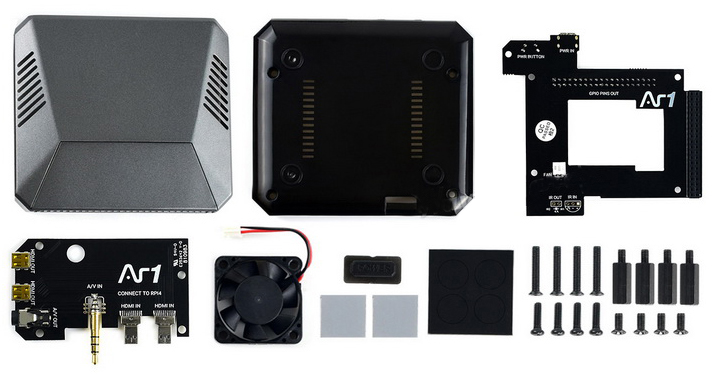
\includegraphics[width=0.8\textwidth]{./Figures/argon2.jpg}
\caption{Partes del gabinete Argon One Pi4 V2 \protect\footnotemark.}
\label{fig:armado}
\end{figure}
\footnotetext{Imagen tomada de \url{https://www.dfrobot.com/product-2090.html}}

\subsection{Sistema operativo para el servidor local}

En la actualidad existen mucha variedad de sistemas operativos para la placa Raspberry Pi, pero para este trabajo se usó el sistema operativo oficial y recomendado por la Raspberry Pi Foundation, llamado ``Raspberry Pi OS'' - version 11 basado en el kernel 5.15.

%La web oficial ofrece diversas versiones a las cuales se puede acceder con descarga directa como se ilustra con la figura \ref{fig:so}.

%\begin{figure}[htbp]
%	\centering
%	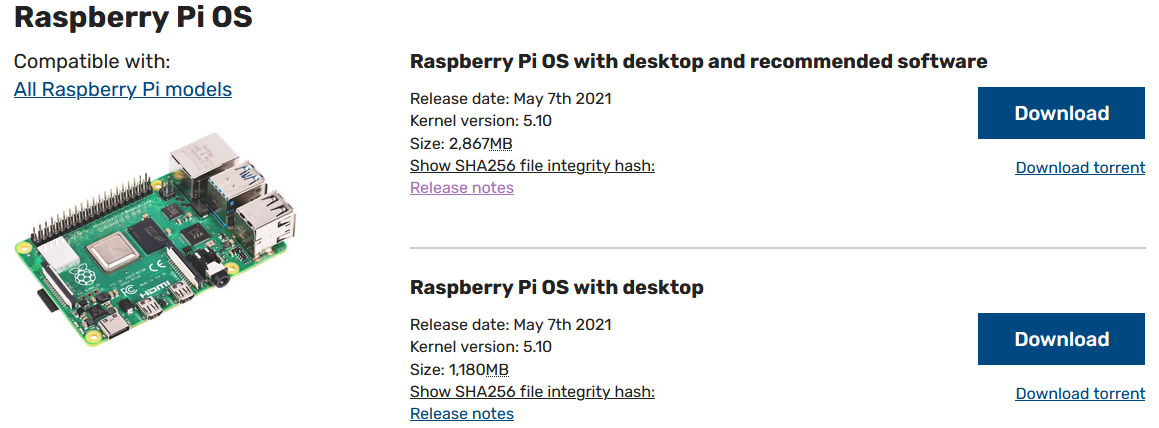
\includegraphics[width=1.0\textwidth]{./Figures/so.png}
%	\caption{Versiones del sistema operativo para Raspberry Pi \protect\footnotemark.}
%	\label{fig:so}
%\end{figure}
%\footnotetext{Imagen tomada de \url{https://www.raspberrypi.com/software/operating-systems/}}

\section{Hardware, sensores y actuadores}

Los componentes principales usados en el desarrollo de cada módulo están formados por una placa base NodeMCU, sensores y actuadores.

\subsection{Placa NodeMCU ESP8266}

La tarjeta NodeMCU es de bajo costo y está basada en el procesador ESP8266, que es muy utilizado en la realización de proyectos IoT, ya que dispone de Wi-Fi integrado. El procesador se programa en Lua \citep{WEBSITE:38}, pero también se puede programar con C/C++. Su principal característica es que trabaja a 3,3 V.  Además, ofrece más ventajas como la incorporación de un regulador de tensión integrado, así como un puerto USB de programación. 

%En el mercado actual se encuentran dos versiones muy utilizadas de la familia NodeMCU y la forma rápida de diferenciar la V2 de la V3, es fijarnos en el conversor serial que monta y en su tamaño. El CP2102 (V2) que es cuadrado, y el CH340G (V3) que es más alargado respectivamente,.
 
Para el trabajo se usó la placa versión 3 del NodeMCU ESP8266 que contiene el driver CH340G requerido para operar el circuito integrado con la interfaz USB. La placa se ilustra con la figura \ref{fig:nodemcu}:

\begin{figure}[htbp]
	\centering
	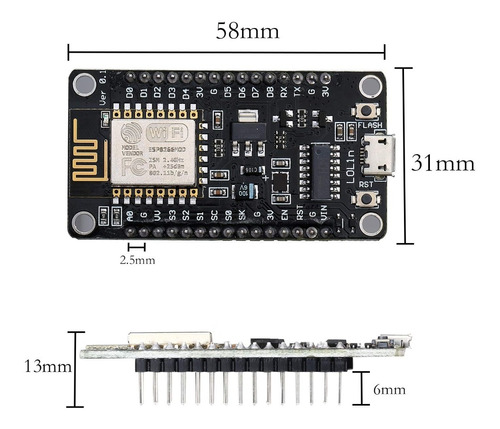
\includegraphics[width=.8\textwidth]{./Figures/nodemcuV3.jpg}
	\caption{Modelo y dimensiones de la placa NodeMCU ESP8266 V3.}

	\label{fig:nodemcu}
\end{figure}

Las especificaciones técnicas del NodeMCU son:

\begin{itemize}
\item Utiliza chip CH340G (USB).
\item Tensión de alimentación: 4,5 V~9 V (10 V max) y/o alimentación por USB.
\item Tensión de pines I/O: 3,3 V.
\item Wireless 802.11 b/g/n standard.
\item Wi-Fi a 2,4 GHz, soporta encriptación WPA/WPA2.
\item Soporta tres modos de operación: STA/AP/STA+AP.
\item Pila de almacenamiento para protocolo TCP/IP (5 conexiones máximo).
\item Pines: D0~D8, SD1~SD3 pueden ser usados como GPIO, PWM, IIC con capacidad de drenar 15 mA por pin.
\item 1 canal ADC: AD0.
\item Consumo de corriente continua ≈ 70 mA (200 mA MAX), Standby: <200 uA.
\item Velocidad de transmisión: 110 - 460800 bps.
\item Soporta interfaz de comunicación UART/GPIO.
\item OTA: \emph{Remote firmware upgrade}.
\item Soporta \emph{Smart Link Smart Networking}.
\item Temperatura de trabajo: -40 ℃ - +125 ℃.
\item Memoria: 4 MByte.
\end{itemize}

\subsection{Sensor de temperatura y humedad DHT11}

El DHT11 es un sensor de humedad relativa y temperatura de media precisión de bajo costo. La salida suministrada es de tipo digital y utiliza solamente un pin de datos. Es usado en aplicaciones académicas relacionadas al control automático de temperatura, aire acondicionado, monitoreo ambiental en agricultura y más. El sensor se muestra en la figura \ref{fig:dht11}.

Utilizar el sensor DHT11 con las plataformas Arduino, Raspberry Pi y NodeMCU es muy sencillo tanto a nivel de \emph{firmware} como \emph{hardware}. A nivel de \emph{software} se dispone de bibliotecas para Arduino con soporte para el protocolo \emph{single bus}. En cuanto al hardware, solo es necesario conectar el pin VCC de alimentación a 3 V - 5 V, el pin GND a tierra y el pin de datos a un pin digital de Arduino \citep{WEBSITE:8}. 

\begin{figure}[htbp]
	\centering
	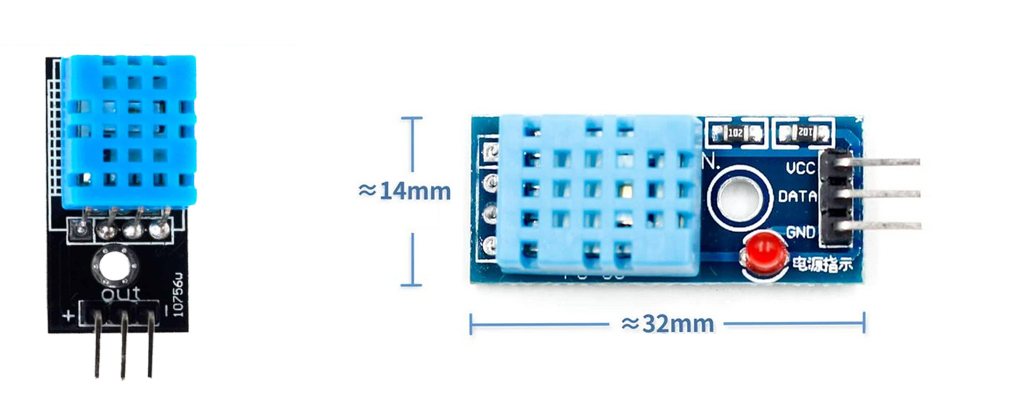
\includegraphics[width=.7\textwidth]{./Figures/dht11.jpg}
	\caption{Modelo y dimensiones del sensor DHT11. }

	\label{fig:dht11}
\end{figure}

Las características más importantes del sensor son:

\begin{itemize}
\item Tensión de operación: 3 V - 5 V DC.
\item Rango de medición de temperatura: 0 a 50 °C.
\item Precisión de medición de temperatura: ±2.0 °C.
\item Resolución temperatura: 0,1 °C.
\item Rango de medición de humedad: 20\% a 90\% RH.
\item Precisión de medición de humedad: 5\% RH.
\item Resolución humedad: 1\% RH
\item Tiempo de sensado: 1 seg.
\item Interface digital: \emph{Single-bus}.
\item Modelo: DHT11
\item Peso: 1 g.

\end{itemize}

\subsection{Sensor de corriente AC SCT-013-030}

La familia de sensores SCT-013 está compuesta por sensores de corriente no invasivo que permiten medir la intensidad que atraviesa un conductor sin necesidad de cortar o modificar el conductor. Estos sensores son usados para medir la intensidad o potencia consumida por una carga eléctrica. Los sensores SCT-013 son transformadores de corriente, dispositivos de instrumentación que hacen posible una medición proporcional a la intensidad que atraviesa un circuito. La medición se realiza por inducción electromagnética \citep{WEBSITE:9}. 

Los sensores SCT-013 disponen de un núcleo ferromagnético partido (como una pinza) que permite abrirlo para arrollar un conductor de una instalación eléctrica sin necesidad de cortarlo, como se ilustra con la figura \ref{fig:sensorCorriente}. Dentro de la familia SCT-013 existen modelos que proporcionan la medición como una salida de intensidad o de tensión. 


\begin{figure}[htbp]
	\centering
	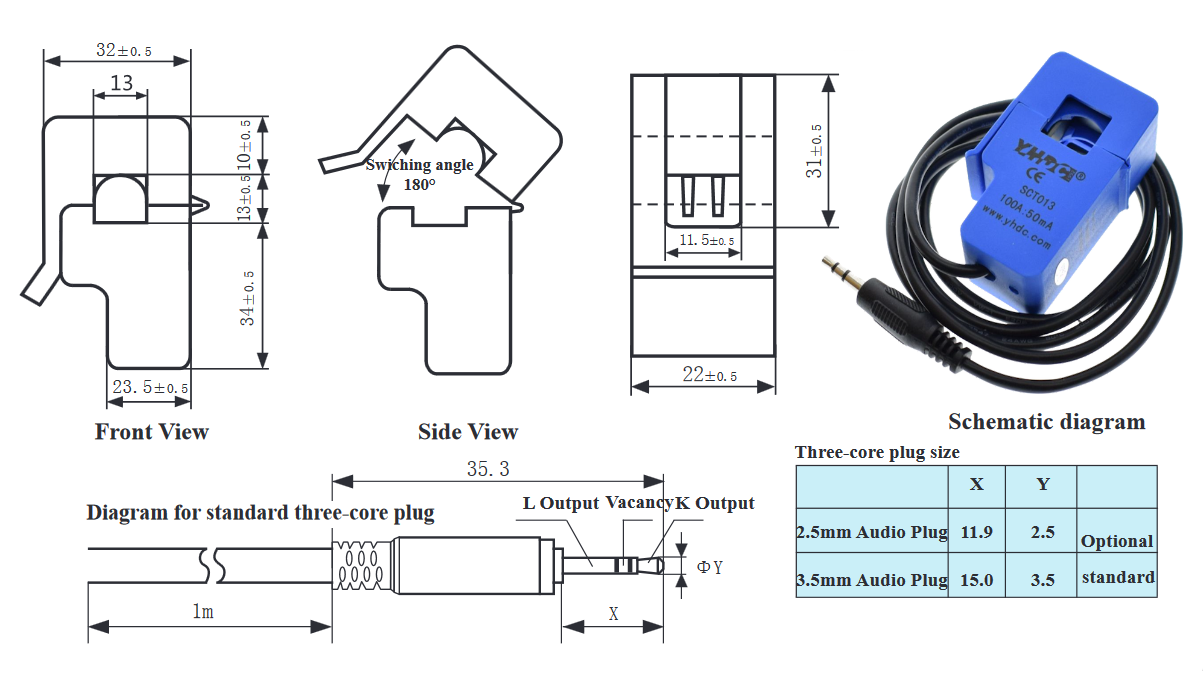
\includegraphics[width=1.0\textwidth]{./Figures/sensorCorriente2.png}
	\caption{Dimensiones del sensor SCT-013-030 AC \protect\footnotemark.}
	\label{fig:sensorCorriente}
\end{figure}

\footnotetext{Imagen de \url{https://datasheetspdf.com/pdf-file/1004704/XiDiTechnology/SCT-013-030/1}}

%El sensor SCT-013 es muy fácil de manejar y acoplar. Puede colocarse como una pinza alrededor de un cable que entre al edificio sin la necesidad de realizar algún trabajo de alta tensión, adecuado para la medición de corriente AC, monitoreo y protección de motores AC, equipo de iluminación, etc \citep{WEBSITE:10}.

Los sensores de la serie SCT-013 son sensores que trabajan como transformadores, la corriente que circula por el cable que se desea medir actúa como el devanado primario (1 espira) e internamente tiene un devanado secundario que dependiendo del modelo puede tener hasta más de 2000 espiras. La cantidad de espiras representa la relación entre corriente que circula por el cable y la que el sensor entrega. Esta relación o proporción es lo que marca la diferencia entre los diferentes modelos SCT-013, adicionalmente pueden tener una resistencia de carga en la salida y de esta forma en lugar de corriente se trabaja con una salida de tensión \citep{WEBSITE:21}. La figura \ref{fig:espiras} ilustra los devanados mencionados:

\begin{figure}[htpb]
\centering 
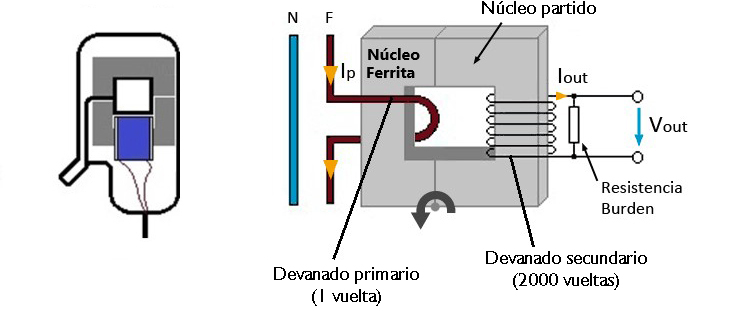
\includegraphics[width=1.0\textwidth]{./Figures/espiras.jpg}
\caption{Partes del núcleo ferromagnético del sensor de corriente.}
\label{fig:espiras}
\end{figure}

Las especificaciones más importantes por las cuales se escogió este instrumento para el desarrollo del trabajo son:

\begin{itemize}
\item Corriente de entrada (inducción): 0-30 A AC.
\item Modo de salida: 0 - 1 V.
\item No linealidad: ±1%.
\item Resistencia (RL): 62 $\Omega $.
\item Grado de Resistencia: Grade B.
\item Temperatura de operación: -25 °C - ﹢70 °C.
\item Longitud del cable: 1 m.
\item Tamaño abierto: 13 mm x 13 mm.
\end{itemize}

%La precisión del sensor puede ser del 1\% a 2\%, pero para ello es muy importante que el núcleo ferromagnético se cierre adecuadamente. Hasta un pequeño hueco de aire puede introducir desviaciones del 10\%. Como desventaja, al ser una carga inductiva, el SCT-013 introduce una variación del ángulo de fase cuyo valor es función de la carga que lo atraviesa, pudiendo llegar a ser de hasta 3º \citep{WEBSITE:9}.

%Los sensores SCT-013 son pequeños transformadores de corriente o CT (\emph{Current transformartor}) instrumentos ampliamente empleados como elementos de medición. Un transformador de corriente es similar a un transformador de tensión y está basado en los mismos principios de funcionamiento. Sin embargo, persiguen objetivos diferentes \citep{WEBSITE:9}.



%La relación de transformación de intensidad se expresa entre el número de espiras, como se muestra en ecuación \ref{eq:proporcionform}.

%\begin{equation}
%	\label{eq:proporcionform}
%	\left( \frac{Is}{Ip} \right)=\left( \frac{Vp}{Vs} \right)=\left( \frac{Np}{Ns} \right)
%\end{equation}

%A esto se le llama relación de transformación. Relaciona el número de espiras del devanado primario (Np), del devanado secundario (Ns), las intensidades del primario (Ip), del secundario (Is), la tensión del primario (Vp) y del secundario (Vs). 


%Para utilizar el sensor SCT-013 no es necesario interrumpir (cortar o desempalmar) el cable a medir, porque al igual que una pinza amperimétrica tiene el núcleo partido. Si se pasa los dos cables de una conexión monofásica, la lectura será 0, puesto que los cables tienen corrientes opuestas \citep{WEBSITE:21}. La figura \ref{fig:conectacorrecto} ilustra la forma correcta de uso del sensor.

%\vspace{0.5cm}
%\begin{figure}[htpb]
%\centering 
%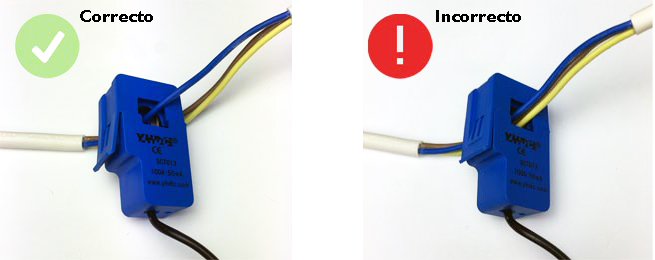
\includegraphics[width=0.8\textwidth]{./Figures/correcto.jpg}
%\caption{Forma de uso del sensor de corriente \protect\footnotemark.}
%\label{fig:conectacorrecto}
%\end{figure}

%\footnotetext{Imagen de \url{https://programarfacil.com/blog/arduino-blog/sct-013-consumo-electrico-arduino/}}


A diferencia de los transformadores de tensión, en un transformador de intensidad el circuito secundario nunca debe estar abierto, porque las corrientes inducidas pueden llegar a dañar el componente. Por este motivo, los sensores SCT-013 disponen de protecciones (resistencia de Burden en los sensores de salida por tensión, o diodos de protección en los sensores de salida por corriente)\citep{WEBSITE:9}.

Para el trabajo se consideró el módulo SCT-013 de 30 A y con soporte para 250 VAC.
%%%%%%%%%%%%%%%%%%%%%%%%%%%%%%%%%%%%%%%%%%%%
\subsection{Sensor de tensión eléctrica AC - ZMPT101B}

El sensor transformador de tensión ZMPT101B permite medir tensión alterna como la que se dispone en la red hogareña. Esta tensión AC no puede ser medida directamente por el ADC del circuito o placa debido a que escapa del rango de entrada (0 V a 5 V). El módulo ZMPT101B soluciona el problema reduciendo la tensión AC de entrada a una tensión menor que pueda ser leída por el Arduino, NodeMCU o cualquier otro microcontrolador. La figura \ref{fig:sensortension} ilustra la forma de conexión del módulo sensor a la línea eléctrica doméstica.

El sensor está integrado por un transformador que cumple la función de aislador galvánico para mayor seguridad en el uso. El lado primario del transformador se conecta a la tensión alterna que se desea medir, por ejemplo la red eléctrica de un hogar de 220 VAC. En el lado secundario del transformador se encuentra un divisor de tensión y un circuito con amplificador operacional (OPAMP LM358) para adicionar un desplazamiento (\emph{offset}) a la salida análoga \citep{WEBSITE:22}. 

\begin{figure}[htpb]
\centering 
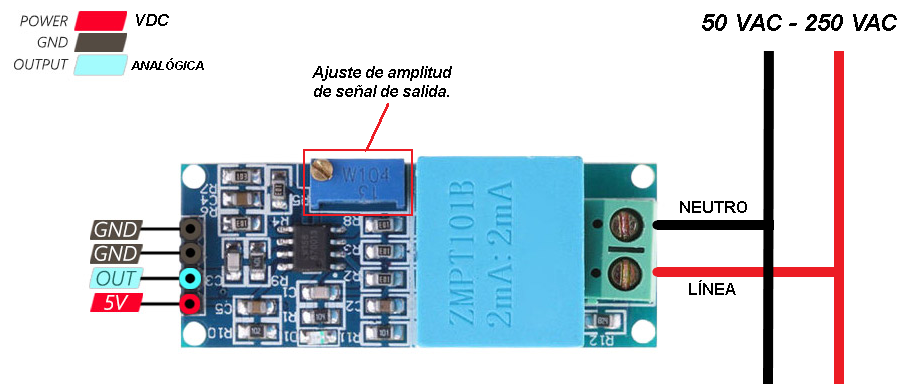
\includegraphics[width=0.85\textwidth]{./Figures/sensortension.png}
\caption{Conexión y partes del sensor de tensión.}
\label{fig:sensortension}
\end{figure}


Este sensor soporta una tensión de entrada de hasta 250 VAC y entrega una onda senoidal de amplitud regulable por un potenciómetro en placa. La onda senoidal de salida está desplazada positivamente para que no tenga tensiones negativas y así poder leerla completamente con el ADC. El desplazamiento depende de la tensión con la que se alimenta el módulo sensor: si la tensión de alimentación es de 5 V el desplazamiento será de 2,5 V y si se alimenta el módulo con 3,3 V el desplazamiento será de 1,65 V \citep{WEBSITE:23}. Su circuito de acondicionamiento de señal interno permite que la tensión de salida del módulo sensor pueda ser leído por cualquier microcontrolador con entrada analógica (ADC). De esta forma, es posible leer la tensión instantánea y realizar cálculos de energía como tensión pico a pico (Vpp) y tensión eficaz (Vrms). 

%Debido a la naturaleza de los transformadores, solo puede medir tensión AC \citep{WEBSITE:22} \citep{ARTICLE:1}. Para su uso con la tarjeta NodeMCU ESP8266, los extremos son 0 y 3.3 V con una compensación de 1.65 V. La figura \ref{fig:ondas} muestra el desplazamiento de onda senoidal.


%\begin{figure}[htpb]
%\centering 
%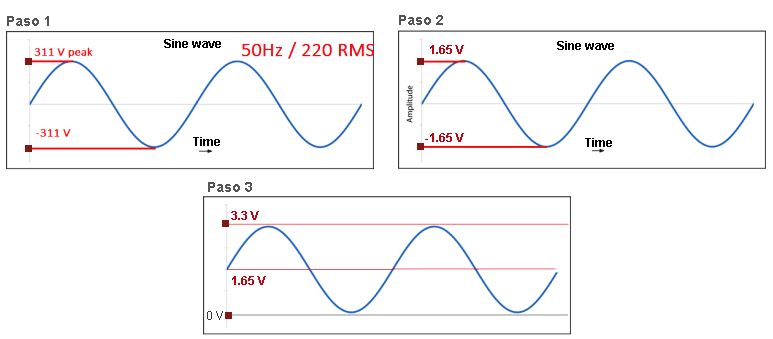
\includegraphics[width=1.02\textwidth]{./Figures/ondas.png}
%\caption{Señal del ZMPT101B con el NodeMCU ESP8266 \protect\footnotemark.}
%\label{fig:ondas}
%\end{figure}

%\footnotetext{Imagen tomada de \url{https://surtrtech.com/2020/04/08/}}

%%%%%%%%%%%%%%%%%%%%%%%%%%%%%%%%%%%%%%%%%%%%



\subsection{Relé Actuador}

Un relé es un interruptor que se puede activar mediante una señal eléctrica. En su versión más simple es un pequeño electro-imán que cuando se lo excita mueve la posición de un contacto eléctrico de conectado a desconectado o viceversa para accionar un circuito mayor. 

Los relés más utilizados son módulos capaces de activarse mediante la entrada de 5 V. La elección de un módulo relé adecuado dependerá de la tensión y amperaje que debe gestionar. En la figura \ref{fig:rele} se aprecian dos modelos de módulos relé con capacidad de activación 5 V y con soporte para 10 A - 250 VAC y 30 A – 250 VAC respectivamente.


\begin{figure}[htbp]
	\centering
	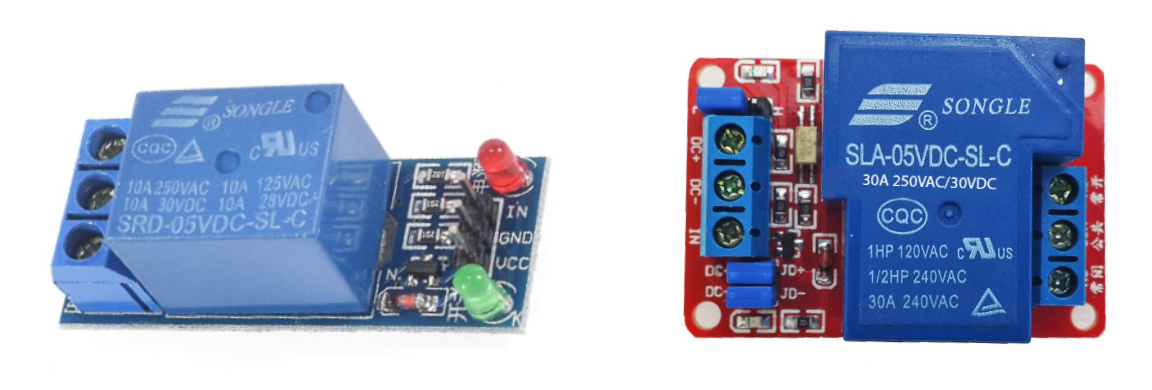
\includegraphics[width=1.0\textwidth]{./Figures/rele.jpg}
	\caption{Modelos de relés con activación de 5 V.}

	\label{fig:rele}
\end{figure}

%El relé es un interruptor que permite trabajar con dos circuitos, uno con tensiones elevadas, por ejemplo, 220 V pero que es activado por un circuito de tensión inferior, por ejemplo, 5 V.

Para el trabajo se consideró el módulo relé de activación 5 V y con soporte para 30 A - 250 VAC.

\subsection{Lenguajes de programación}

La elaboración de este trabajo involucró el usó de distintos \emph{software}s como herramientas para facilitar el desarrollo, así como el uso de diversos lenguajes de programación que se describen a continuación:
\begin{itemize}
\item Python: es un lenguaje de programación interpretado cuya filosofía hace hincapié en la legibilidad de su código. Se trata de un lenguaje de programación multiparadigma, ya que soporta parcialmente la orientación a objetos, programación imperativa y, en menor medida, programación funcional.

Se utilizó para la creación de procesos internos en el módulo principal. 
\item PHP: es un lenguaje de programación de uso general que se adapta especialmente al desarrollo web del lado del servidor.

Se utilizó como lenguaje \emph{backend} del \emph{software} de monitoreo y control.
\item JavaScript: lenguaje de programación interpretado utilizado en el lado del cliente. Es el único lenguaje de programación que funciona en los navegadores de forma nativa.

Se utilizó como lenguaje frontend del \emph{software} de monitoreo y control.
\item Arduino: lenguaje de programación que está basado en C++.

Se utilizó como lenguaje para programar el firmware de los módulos de sensores y actuadores.
\end{itemize}